\section{}
Consider a pendulum consisting of a mass $M$ on a thin (nearly massless) rod with length $L$. 
An input torque $\tau$ is applied at the pivot point of the pendulum. The angle $\theta$ 
measures the deflection of the pendulum away from the vertical.


\begin{figure}[h]
    \centering
    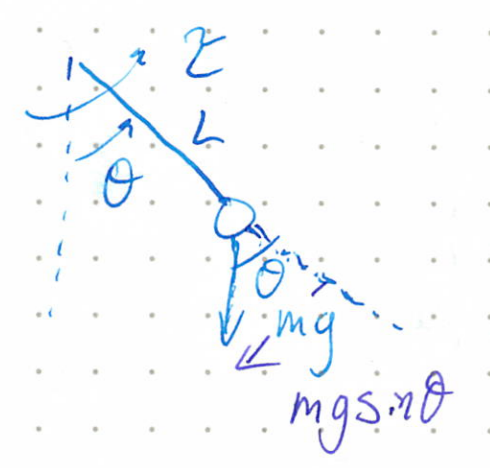
\includegraphics[width=0.5\textwidth]{Questions/Figures/Q1fbd.png}
    \caption{Pendulum free-body diagram.}
    \label{fig:Q1fbg}
\end{figure}

\subsection{}
\textit{Starting from a free-body diagram, obtain the equation of motion of the system. (Note: $J = ML^2$ is the mass moment of 
inertia of the pendulum about its pivot point).}

Taking the moment at the pivot point of the pendulum, we have
\[
    \begin{aligned}
        \circlearrowleft \sum M &= J\ddot{\theta} = \tau - MgL\sin\theta \\
        \implies ML^2\ddot{\theta} &= \tau - MgL\sin\theta \\
         \ddot{\theta} &= \boxed{\frac{\tau}{ML^2} - \frac{g}{L}\sin\theta}
    \end{aligned}
\]

\subsection{}
\textit{Put the ODE into the state dynamics form $\dot{x} = f(x, u)$.}

Let $x = [\theta, \dot{\theta}]$, then
\begin{empheq}[box=\fbox]{align*}
        \dot{x} &= \begin{bmatrix}
            x_2 \\
            \frac{\tau}{ML^2} - \frac{g}{L}\sin x_1
        \end{bmatrix} 
\end{empheq}

\subsection{}
% Taking the parameter values M = 0.2 kg, L = 0.5 m, g = 9.81 m/s2
% and input τ (t) = 0.1 sin t,
% obtain a plot of the response θ(t) for 0 ≤ t ≤ 10 given initial conditions θ(0) = π/6 rad,
% ˙θ(0) = −1 rad/s. Submit your plot plus the .m function you used.

\textit{Taking the parameter values $M = 0.2$ kg, $L = 0.5$ m, $g = 9.81$ m/s$^2$ and input $\tau(t) = 0.1 \sin t$, 
obtain a plot of the response $\theta(t)$ for $0 \leq t \leq 10$ given initial conditions 
$\theta(0) = \frac{\pi}{6}$ rad, $\dot{\theta}(0) = -1$ rad/s. Submit your plot plus the .m function you used.}

% Plot 
\begin{figure}[h]
    \centering
    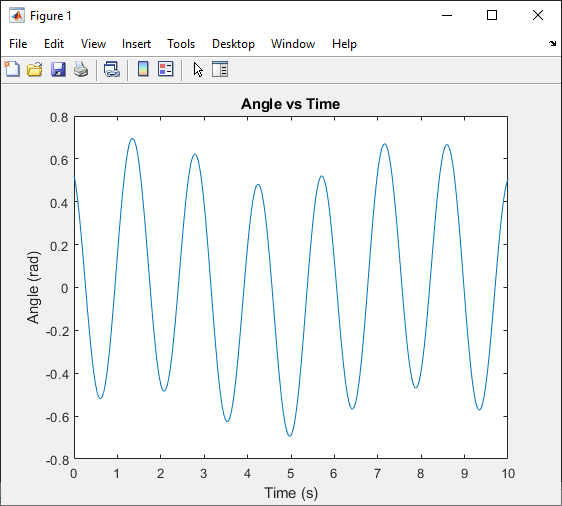
\includegraphics[width=0.8\textwidth]{Questions/Plots/Q1CAngleVsTime.png}
    \caption{Plot of $\theta(t)$ for $0 \leq t \leq 10$ given initial conditions}
    \label{fig:Q1c}
\end{figure}

\begin{figure}[h]
    \centering
    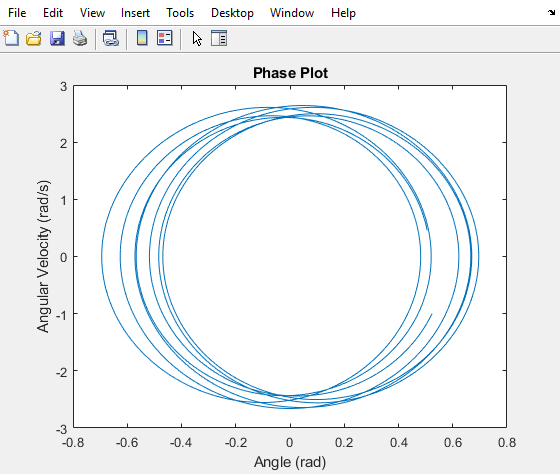
\includegraphics[width=0.8\textwidth]{Questions/Plots/Q1CPhasePlot.png}
    \caption{Phase portrait of $\theta(t)$ for $0 \leq t \leq 10$ given initial conditions}
    \label{fig:Q1cPhasePortrait}
\end{figure}

\FloatBarrier

The Matlab code used to generate the plots is:

\lstinputlisting[language=Matlab]{Questions/Code/a2q1.m}


% \subsection{}
% \textit{What is a disturbance for this system?}

% For this system, a disturbance are environmental factors that affect the temperature of the BBQ, such as wind, rain, ambient temperature, etc.

% \subsection{}
% \textit{Draw a block diagram of the overall closed-loop system. Label the signal arrows and name
% the controller, actuator, plant and sensor in your diagram.}

% \begin{figure}[h]
%     \centering
%     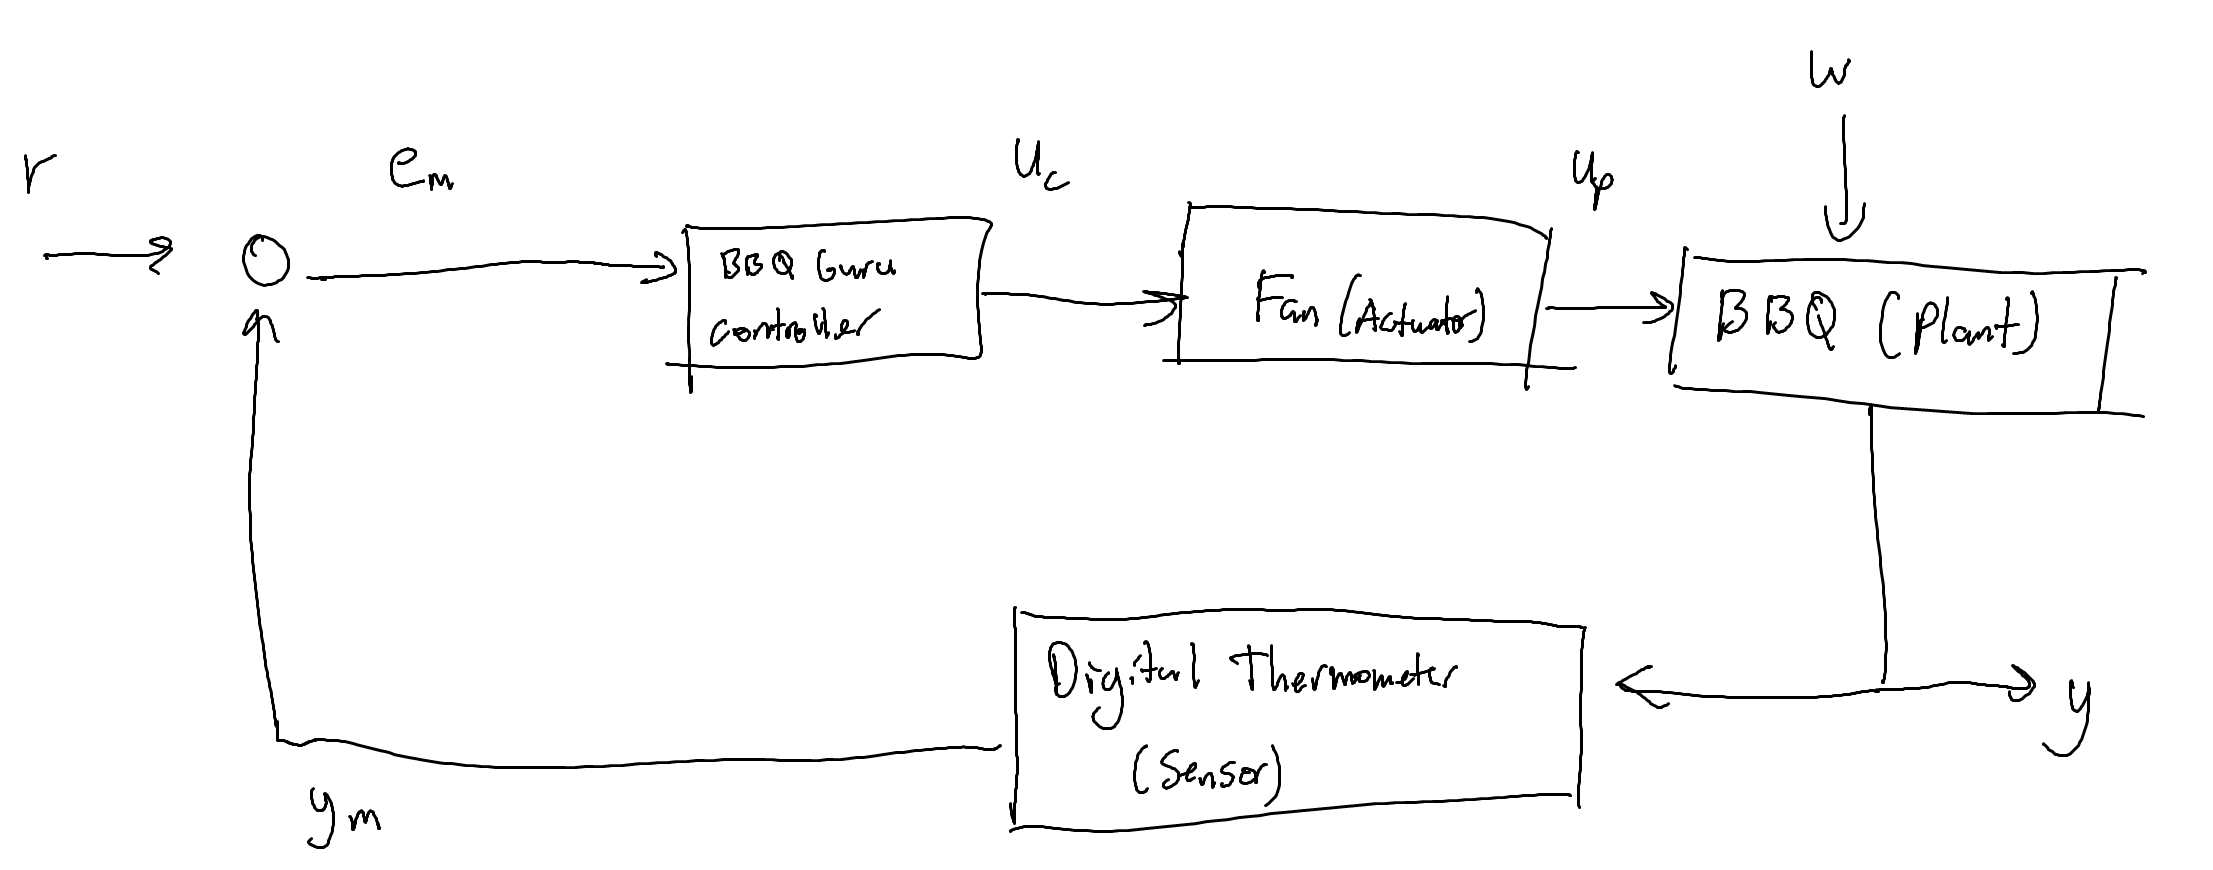
\includegraphics[width=0.8\textwidth]{Questions/Figures/Q1c.png}
%     \caption{Block diagram of the overall closed-loop system for BBQ Guru.}
%     \label{fig:Q1c}
% \end{figure}

% Where
% \begin{itemize}
%     \item $r$ is the reference signal, the desired temperature of the BBQ
%     \item $e_m$ is the measured tracking error, the difference between the desired temperature and the measured temperature of the BBQ
%     \item $u_c$ is the control input, which is the output of the controller to the fan 
%     \item $u_p$ is the plant input, which is the fan speed which controls the amount of oxygen supplied to the charcoal, affecting the temperature of the BBQ
%     \item $y$ is the plant output, the actual temperature of the BBQ
%     \item $y_m$ is the measured plant output, the measured temperature of the BBQ from the temperature sensor as an electronic signal
%     \item $w$ is the disturbance, which is the environmental factors that affect the temperature of the BBQ
%     \item $v$ is the sensor noise, which is the noise from the temperature sensor
% \end{itemize}
